\section{Problem \& Needs}
\subsection{Scenario Definition}
Our problem and driving dilemma of our project is to develop \textbf{An imaging system that can be used for space observation}. 
\vspace{2mm}

\subsection{User Needs \& Requirements}
\subsubsection{User Needs}
User needs can be defined as the needs that a user has for a particular service. The service must satisfy the user's needs to get the right outcome or result from the product \cite{GOVUK2023}. The purpose of defining the user needs is to capture what we want to achieve with our design. The 'user needs' allow us to capture the user, keeping our customer at the heart of our design. It aids in aligning the team and the final product to a concise vision. The needs also provide us with a benchmark for success and will help us verify our design by comparing them against the statements. The user needs were developed by setting the scope with a problem statement and then researching our customers.
\vspace{1.5mm}

When developing user needs our main consumer was from a research background. The most common users of the Hubble Telescope, which our concept derives from, were astronomers who would use the satellite for space observation. We also see from their international partnerships NASA also allowed scientists to use the satellite as they guaranteed ESA 15\% of Hubble's observing time \cite{NASA2023}. Although the user needs were derived with astronomers in mind these needs also satisfy our expected customers like scientists, researchers from university backgrounds and also larger organisations such as NASA and ESA. The 'user needs' allow us to adhere to a wider market but also solve our problem.
\vspace{1.5mm}

The philosophy behind the user needs is to identify the user, and then look at the need and what they expect to achieve from the product. The user needs are identified in Table \ref{tab:User Needs} below. 

\begin{table}[H]
\centering
\begin{tabular}{|l|c|}
\hline
\textbf{Need} & \textbf{Need Statement}                                                                                                                   \\ \hline
\textbf{N1}        & The user needs a way of localizing multi-agent UAVs in GNSS denied environment.

\\ \hline
\textbf{N2}      & The user shall receive processed coordinates in Body \& Inertial Coordinate.\\ \hline
\textbf{N3}        & The user shall have the ability to receive desired/request sensors data                                                                                                       \\ \hline
\end{tabular}
\caption{Subsystem Needs}
\label{tab:User Needs}
\end{table}

\subsubsection{User Requirements}
% Please add the following required packages to your document preamble:
% \usepackage{graphicx}
\begin{table}[H]
\centering
\resizebox{\columnwidth}{!}{%
\begin{tabular}{|l|c|l|}
\hline
\multicolumn{1}{|c|}{\textbf{\begin{tabular}[c]{@{}c@{}}User \\ Requirement\end{tabular}}} & \textbf{Description}                                                                                                                                                 & \textbf{User Need} \\ \hline
\textbf{UR1}                                                                               & The user shall be able to recieve high resolution images of at least 0.025 arcseconds per pixel                                                                      & N1                 \\ \hline
\textbf{UR2}                                                                               & The satellite shall be sustainable                                                                                                                                   & N5                 \\ \hline
\textbf{UR3}                                                                               & \begin{tabular}[c]{@{}c@{}}The user needs to be able to interact with the system to request specific images or \\ communicate for mission coordination.\end{tabular} & N1, N3, N10        \\ \hline
\textbf{UR4}                                                                               & The user shall be able to receive an image requested from the satellite in less than a year.                                                                         & N4                 \\ \hline
\textbf{UR5}                                                                               & The user shall be able to communicate with the company to coordinate images                                                                                          & N3                 \\ \hline
\textbf{UR6}                                                                               & The user shall be able to view stars at least 10-15 billion light years away                                                                                         & N1 N8              \\ \hline
\textbf{UR7}                                                                               & The user shall receive stable images without distortion                                                                                                              & N3                 \\ \hline
\textbf{UR8}                                                                               & \begin{tabular}[c]{@{}c@{}}The user shall be able to rely on the system for long-term observations, at least\\ 15 years\end{tabular}                                 & N5, N7             \\ \hline
\textbf{UR9}                                                                               & The system shall provide near real-time imaging.                                                                                                                     & N4                 \\ \hline
\textbf{UR10}                                                                              & The satellite shall have a field of view of at least 2.7 arcminutes by 2.7 arcminutes                                                                                & N9                 \\ \hline
\textbf{UR11}                                                                              & The user shall be able to obtain images that view UV light, Visible light and near-infrared                                                                                                & N2                 \\ \hline
\end{tabular}%
}
\caption{User Requirements }
\label{tab:User Requirements }
\end{table}
\subsubsection{User Requirement Justifications} \label{User Requirement Justifications}
\textbf{UR1}: 
The benchmark for our satellite is the Hubble Telescope. Astronomers use the Hubble telescope for research and its high quality allows the user to conduct detailed analyses of distant bodies and star formations. Quality is important when using the telescope making it a crucial user need.\\
\vspace{1.5mm}

\textbf{UR2}:
Sustainability is important when it comes to the space industry. It is a major concern to astronomers and researchers in the field. By minimising harmful materials and designing for safe end-of-life disposal. A sustainable satellite can reduce the need for costly repairs and servicing missions. We can focus on durability and effective use of resources.\\
\vspace{1.5mm}

\textbf{UR3}:
For the telescope to be useful to the user, the user must be able to request desired images, images of a certain constellation or galaxy, and also be able to receive them and view them. This means that a system should be put in place where the telescope can be manoeuvred and images can be sent to ground control and processed.\\
\vspace{1.5mm}

\textbf{UR4:}
The Hubble team took at least a year to receive, process and distribute images from the telescope. Researchers and astronomers need to be able to receive images as soon as possible to aid the development and cut down on lead times so this 'user need' was derived to ensure we are meeting similar performance criteria. Also from a market perspective, this will make our telescope favourable for use.\\
\vspace{1.5mm}

\textbf{UR5}: To meet \textbf{N3} the user requires a system that will allow them to interact with the telescope which will happen through the company. Making this a requirement ensures that we put in a system in our operations which will allow the customer to request and receive desired images.

\textbf{UR6}: This user requirement was derived from the performance of the Hubble Telescope as it was used mainly for its range, this user requirement ensures that we meet the same performance criteria.\\
\vspace{1.5mm}

\textbf{UR7}: \textbf{N3} specifies that the customer should be able to receive '\textit{desired images}', developing this need produced \textbf{UR7}. If the customer requests specific coordinates or a certain constellation, the satellite should be able to correct itself and point in the desired position much like the Hubble \cite{NASA2023_Img}. This also means that we have to ensure pointing for long periods for the image to be clear and uninterrupted. This also links into the structure of our communication system and onboard storage which are further discussed in our sub-system requirements \\
\vspace{1.5mm}

\textbf{UR8}: Most modern satellites are built to last many years. By focusing on a long life span it provides uninterrupted data for long-term astronomical projects. By design a system that has long-term use maximises the return on investment, it also results in fewer failures or downtimes since it is built for long-term use.\\
\vspace{1.5mm}

\textbf{UR9}: Real-time data links with \textbf{N3}, it is crucial for observing the rapidly changing events that take place in space. Near real-time imaging allows us to capture data that might otherwise be missed which can provided valuable information for further research. Immediate access to data also reduces the need for multiple redundant images, as scientists can compile and verify photos quickly. 

\textbf{UR10}: This field of view requirement stems from the Hubble Telescope's current performance. The Hubble has a field of view of 2.7 arcminutes by 2.7 arcminutes \cite{STScI2023}, having a larger field of view means that more subjects can be included in the captured images. Since we are looking to produce a replacement for Hubble the user will need a system of similar performance. This user need, like many other user needs stems from Hubble's current performance.\\
\vspace{1.5mm} 

\textbf{UR11}: The Hubble telescope collects UV light, Visible light and near-infrared \cite{NASA2023_W}. Using this criteria \textbf{N2} was developed. The 'and/or Infrared' clause was derived from Hubble's main use to view the visible light spectrum. It only collected some UV and IR wavelengths. If astronomers wanted to view IR imaging then they would opt for more purpose-built satellites like the James Webb telescope, which was made for Infrared wavelengths.\\
\vspace{1.5mm}

\subsection{Market Analysis}
\subsubsection{Costumers and Competitors}
Within the market, the top competitors for a deep space imagery satellite are identified to be: 
\begin{enumerate}
    \item \textbf{National Aeronautics and Space Administration (NASA):} Based in the United States, NASA has launched numerous space telescopes, including the groundbreaking James Webb Space Telescope (JWST). Currently, NASA is developing the Habitable Worlds Observatory (HWO), designed to search for and study exoplanets within the habitable zone—also known as the "life region"—where conditions might support life \cite{NASA_HWO}. User requirement N10 specifies a similar objective for our conceptual satellites. However, unlike HWO, the main objective of our satellite is not solely exoplanet imagery but rather deep space imagery. NASA's most recent launch JWST has been celebrated worldwide as a marble of engineering science and their future work is likely to follow \cite{Pacucci2023}. It is important to consider that the concepts proposed later in the report must account for JWST to ensure enough social, scientific, and economic attraction. 
    
    \item \textbf{European Space Agency (ESA):} Headquartered in France, the European Space Agency (ESA) has launched a total of 11 space telescopes, with its most recent mission, Euclid, launched on July 1, 2023. Euclid’s primary goal is to map the geometry of the dark Universe by observing in the visible and near-infrared wavelengths, which allows it to study dark matter and dark energy across billions of galaxies \cite{ESA_Euclid}.
\vspace{1.5mm}

Although ESA does not currently operate any telescope that meets the user needs outlined above, it remains a significant competitor due to its substantial investments and collaborative contributions to major space missions. Notably, ESA played a key role in the JWST project by providing the Ariane 5 rocket \cite{ESA_Ariane5} used for JWST’s launch and two critical instruments onboard \cite{Gardner2006}: NIRSpec (Near-Infrared Spectrograph) and MIRI (Mid-Infrared Instrument). These instruments are essential for deep-space observations, including the analysis of distant galaxies and the atmospheres of exoplanets.
    \item \textbf{Japan Aerospace Exploration Agency (JAXA):} Although JAXA currently has no prominent active deep space imaging satellites, the agency has a history of developing such technology, as demonstrated by the planned LiteBIRD mission \cite{LiteBIRD2024}. This mission, set for launch in the early 2030s (similar to our 2029 expected launch), exemplifies JAXA's commitment to advancing space imaging capabilities over the next 5-10 years.

    \item \textbf{China National Space Administration (CNSA):} With substantial investment from the Chinese government, the CNSA conducts frequent satellite launches. A notable upcoming mission, planned for 2026, will place a deep-space imaging satellite equipped with a 2-meter diameter primary mirror into orbit. This telescope, with a field of view 300-350 times larger than the Hubble Space Telescope, represents a significant advancement in space imaging technology \cite{CNSA2026}. While this satellite is the most capable competitor among those mentioned and will be operational within five years, political restrictions may limit access for U.S. and potentially EU users, thereby sustaining demand for a successor to the HST.
\end{enumerate}
\noindent We consider only main organisations for competition due to the scenario definition. Based on the user needs identified, the customers identified are:
\begin{enumerate}
    \item \textbf{Research Institutions}: A report by the Space Academic Network (SPAN) identified approximately 2,000 university-based researchers focused on space science within the UK alone. Comparable estimates may apply to other active nations in space research, including the USA, France, Germany, and Spain, as well as additional EU countries \cite{ESPI2022}. Furthermore, the field of astronomy is projected to grow by 7\% from 2023 to 2033, indicating a rising demand for advanced astronomical telescopes \cite{BLS2023}.
    \item \textbf{Space Agencies and Government bodies}: NASA, ESA, UK Space Agency all would likely be very interested in high-quality imagery for scientific purposes and may even support financially. 
    \item \textbf{Commercial Enterprises}: Aerospace defence companies and telecommunications operators may also show their interest in space imagery to gain value experience on orbital debris, space weather and other space-phenomena. 
    \item \textbf{Non-Profit and International Organizations}: these include, but are not limited to, the International Astronomical Union (IAU), which may fund space research and facilitate access for member institutions or countries with limited space programs.
\end{enumerate}



\subsubsection{Space Market Review and Future Forecasts}
As of June 2024, there are estimated to be around 10,000 active satellites orbiting Earth \cite{SpaceWatch2024}, with the global space industry projected to grow to \$1.8 trillion by 2035. This shows that the space industry will become even more prominent in the future, and that sustainability must be considered.\\
\vspace{1.5mm}

The most prominent space telescopes are NASA's Hubble Space Telescope and the James Webb Space Telescope, a joint venture between NASA and ESA. Both of these telescopes provide astronomical research institutes with invaluable resources. Other smaller telescopes are active, observing the universe under different spectrums, such as Fermi \cite{fermi_gamma_ray_space_telescope} and NuStar \cite{nustar}.  A new competitor is set to join the market in 2026, in the form of the Xuntian, a space telescope launched by the Chinese Manned Space Agency \cite{XuntianDelay}. Due to policies from the UK government concerning the use of Chinese-based services, the Xuntian should not pose as a significant competition to our concept \cite{gov2024china}. \\
\vspace{1.5mm}

There is an increased demand for planetary and deep space observation, primarily caused by the James Webb space telescope launch. A 2023 discovery of carbon dioxide and methane in a distant exoplanet emphasises the importance of deep space observation \cite{nasa2023webb}.\\
\vspace{1.5mm}

Commercial players have also begun to enter the deep-space telescope market, mainly taking the form of collaborations with established space agencies such as NASA, ESA, and JAXA to both reduce the cost as well as foster technological advancement \cite{nasa2023collaboration}.
\begin{figure}[h]
    \centering
    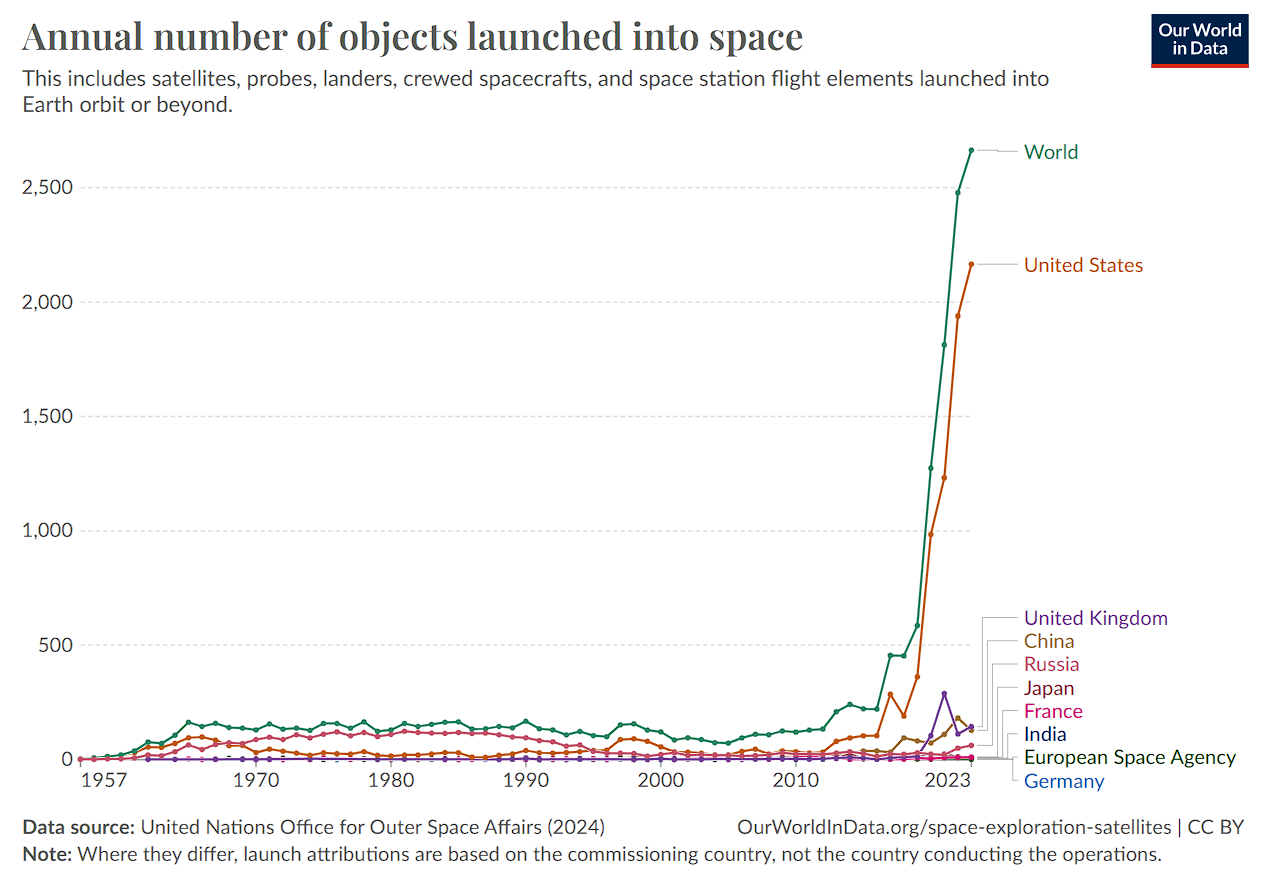
\includegraphics[width=0.75\linewidth]{Screenshot 2024-11-06 140945.png}
    \caption{Yearly Number of Launches \cite{OurWorldInData2024}}
    \label{fig:enter-label}
\end{figure}
The market landscape for deep space observation satellites reflects the overall increased need for scientific, commercial and space research from the government. The rise in interest in space research from both government agencies and the private sector. NASA and ESA alongside various private entities, makes up 65\% of current satellite launches and manufacturing in 2023 \cite{Erwin2023}.\\
\vspace{1.5mm}

There is a constrained yet still competitive market in terms of launch options. The recent surge in private manufacturers of launch vehicles has reduced the prices required to launch satellites into orbit. SpaceX has become one of the leading providers of launch systems, accounting for 45\% of global launches in 2023 \cite{USITC2021}. As a result, prices for SpaceX launches can reach as low as \$1,400 per Kg for the SpaceX Falcon Heavy \cite{SpaceXprice}, compared to the \$43,000 per Kg offered by NASA's SLS \cite{SpaceImpulse2023}.\\
\vspace{1.5mm}
